\subsubsection{Profibus}\label{par:profibus}
\paragraph{Краткое резюме}
\pb -- один из самых популярных и широко применяемых протоколов при автоматизации. Протокол работает по такой же системе, что и \mb: master -  slave. 

Этот протокол используется для передачи полевых данных в системы уп\-равления технологическими процессами и обеспечивает прямое управление и обслуживание устройств. При смене полевого устройства новое устройство автоматически берет на себя роль предыдущего устройства, что позволяет легко осуществлять смену устройств без прерывания работы системы.

Существует 3 подвида \pb \cite{__2001, __2002, galloway_introduction_2012}:
\begin{enumerate}
	\item \pb \textit{DP}: быстрый протокол с одним мастером. Обеспечивает высокую скорость передачи данных (до $12$ Мбит/с). Отлично подходит для построения систем контроля и сбора данных с одним ведущим узлом. Работает на низком уровне;
	\item \pb \textit{FMS}: предназначен для работы с системами производителей, не поддерживающих \pb \textit{DP} \cite{__2001, promwad__2019-1};
	\item \pb \textit{PA}: используется во взрывоопасных местах. Подключается к \newline \pb \textit{DP} через разветвители.
\end{enumerate}
\paragraph{Принцип работы}\label{par:pb_work}
\pb как и \mb работает по протоколу master - slave. Однако, в отличие от \mb, этот протокол способен работать с несколькими мастерами благодаря кольцевой топологии (см. \refpar{par:topology}) и маркерному доступу \cite{powell_profibus_2013}.

Каждое устройство должно пройти через ``инициализацию'', во время которой оно подключается к сети. У каждого ведомого устройства есть ``таймер отказоусточивости'' -- если мастер не разговариал с ним некоторое время, устройство возвращается в ``спячку'' и ему придётся повторить процедуру инициализации снова. В комбинации со сторожевым таймером это даёт гарантию того, что передача данных будет происходить каждый ``цикл''.

Цикл проходит так (см. \refris{fig:profibustoken}): мастер А получает токен, опрашивает своих подопечных и передаёт токен дальше. 

\begin{figure}
	\centering
	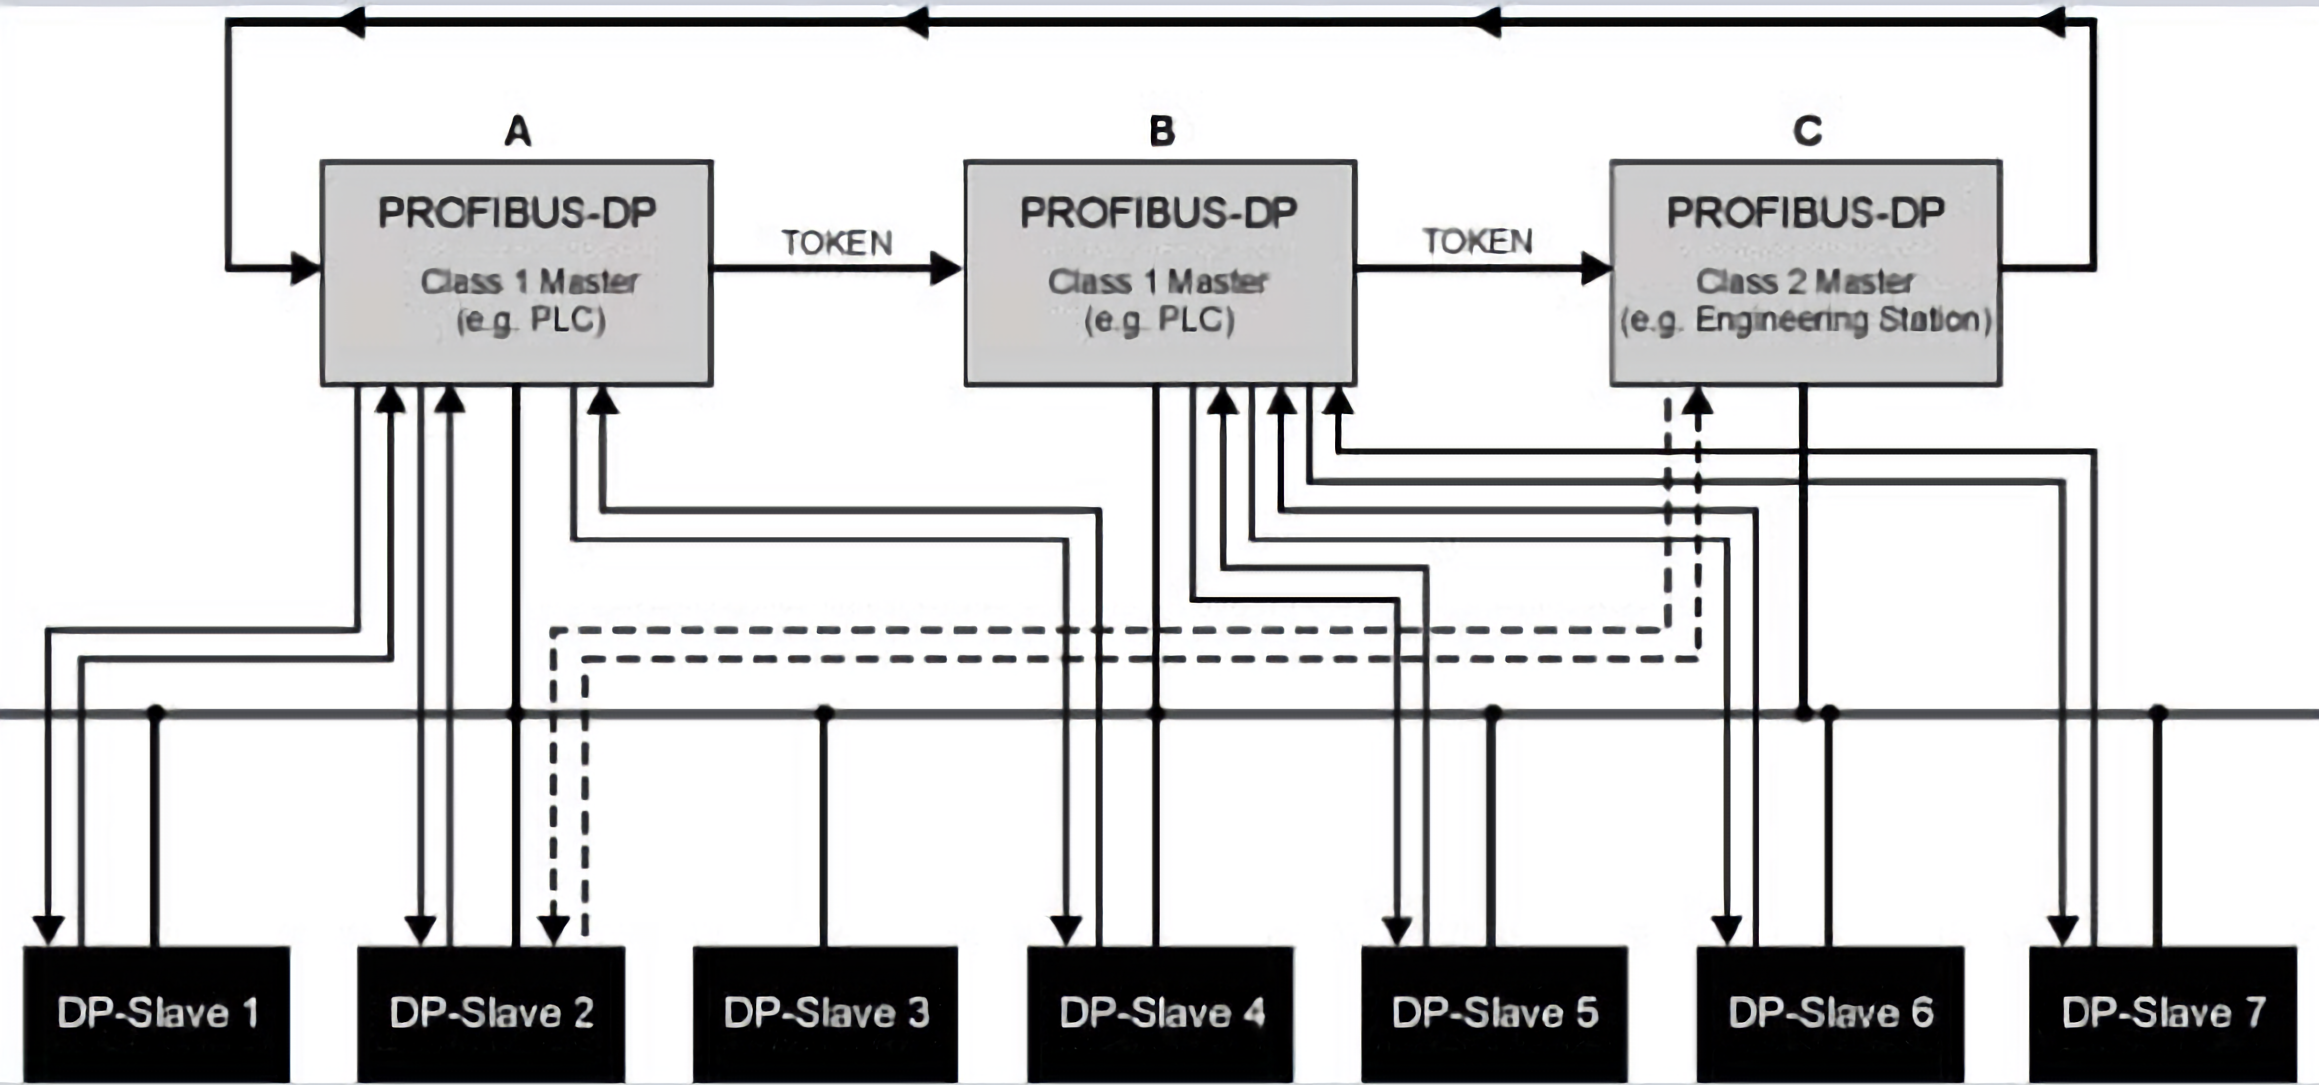
\includegraphics[width=0.9\linewidth]{images/profibus_token}
	\caption{Цикл \pb}
	\label{fig:profibustoken}
\end{figure}

\subparagraph{Физический уровень}
На физическом уровне \pb использует стандарт RS-485 при скорости передачи до 12 Мбит/с и с размерами сегментов сети до 32 устройств. Количество устройств можно увеличить с помощью повторителей интерфейса \cite{powell_profibus_2013}.

Протокол устойчив к помехам и шумам. В случае правильной установки и настройки представляет из себя сверхнадёжную систему \cite{powell_profibus_2013}.

\subparagraph{Канальный уровень}
Обеспечиваются следующие требования:
\begin{itemize}
	\item в процессе коммуникации между ведущими устройствами необходимо обеспечить выполнение каждым из них своей задачи в течение заранее определенного интервала времени;
	\item взаимодействие ведущих устройств (контроллеров) с ведомыми должно происходить максимально быстро.
\end{itemize}

Используемый в протоколе метод передачи маркера по кольцу показан на \refris{fig:profibustoken}.
\subparagraph{Передача сообщений}
У \pb есть два типа сервисов передачи сообщений \cite{__2015}:
\begin{enumerate}
	\item \textbf{SRD}: позволяет отправить и получить данные в одном цикле обмена. Этот способ обмена наиболее распространен в \pb и очень удобен при работе с устройствами ввода-вывода, поскольку в одном цикле можно и отправить и получить данные;
	\item \textbf{SND}: используется, когда надо отправить данные одновременно группе ведомых устройств (многоабонентский режим) или всем ведомым устройствам (широковещательный режим). При этом ведомые устройства не отправляют свои уведомления мастеру.
\end{enumerate}

Пакет данных в \pb называется телеграмма. Её структура приведена на \refris{fig:profibustg}
\begin{figure}
	\centering
	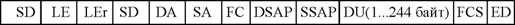
\includegraphics[width=\linewidth]{images/profibus_tg}
	\caption{Структура телеграммы \pb}
	\label{fig:profibustg}
\end{figure}
Расшифровка полей телеграммы \cite{__2015, acromag_introduction_2002}:
\begin{itemize}
	\item \textbf{SD:} стартовый разделитель. Используется для указания начала телеграммы и ее формата;
	\item \textbf{LE:} длина передаваемых данных (DA+SA+FC+DSAP+SSAP+DU);
	\item \textbf{LEr:} повторение поля LE с целью его резервирования;
	\item \textbf{DA:} адрес устройства-получателя телеграммы;
	\item \textbf{SA:} адрес отправителя;
	\item \textbf{FC:} код типа телеграммы (запрос, уведомление, ответ, диагностические данные, тип устройства - мастер или ведомый, приоритет, уведомление);
	\item \textbf{DSAP:} устройство-получатель использует это поле, чтобы определить, какой тип сервиса нужно выполнить;
	\item \textbf{SSAP:} COM порт отправителя;
	\item \textbf{DU:} данные длиной от 1 до 244 байт;
	\item \textbf{FCS:} контрольная сумма телеграммы (сумма значений полей DA+SA+ FC+DU, по модулю 255);
	\item \textbf{ED:} признак конца.
\end{itemize} 

\paragraph{Profinet}
Как и у \mb, у \pb есть аналог для работы с сетью. Только в отличие от инкапсулирования обычного пакета в \tcp, \textit{Profinet} -- протокол, который был разработан для того, чтобы использовать все преимущества сети \textit{Ethernet} (включая такую функцию, как \textit{Profisafe}) \cite{powell_profibus_2013}.

Более подробно с протоколами семейства \pb можно ознакомиться в документации стандарта \cite{acromag_introduction_2002}.